\documentclass[11pt,a4paper]{article}

% ------------------------------------------------------------------ packages
\usepackage[margin=2.5cm]{geometry}   % page margins
\usepackage{amsmath, amssymb}         % mathematics
\usepackage{graphicx}                 % figures
\usepackage{booktabs}                 % clean tables
\usepackage{float}                    % [H]: figure exactly where it is written
\usepackage[hidelinks]{hyperref}      % clickable references and links

\graphicspath{{../figures/}}          % figures are produced by the code

% ------------------------------------------------------------------ title
\title{Double Descent in Linear Models}
\author{Andrea Vaselli\\[2pt]
        \small Statistical Methods for Machine Learning, A.Y.\ 2025/26\\
        \small Code: \url{https://github.com/andreavase27/double-descent-linear-models}}
\date{}
\begin{document}
\maketitle

% =================================================================== ABSTRACT
\begin{abstract}
Following Belkin et al., we study the \emph{double descent} curve in
linear regression, fixing the number of training points ($n = 100$) and
varying the number of features $d$. We compare minimum-norm least squares
and ridge regression on synthetic data with noisy linear labels and on the
California Housing dataset. In every setting the test error peaks exactly
at the interpolation threshold $d = n$, together with the norm of the
coefficients, and decreases again beyond it; on synthetic data this
matches a closed-form expression for the expected error. Whether overparameterized
models beat the classical ones depends on how the signal is spread across
the features, and ridge regression with a cross-validated penalty removes
the peak. As extensions, we show that gradient descent started at zero
converges to the minimum-norm solution and that the peak grows with the
label noise.
\end{abstract}

% =================================================================== 1
\section{Introduction}

The classical view of generalization is built on the bias--variance
trade-off. A model that is too simple cannot capture the structure of the
data (high bias), while a model that is too complex starts fitting the noise
(high variance), so the test error follows a U-shaped curve. A direct
consequence is that a model with zero
training error, one that interpolates the data, should generalize poorly.

Modern machine learning does not seem to follow this rule. Large models,
such as neural networks with far more parameters than training points, are
routinely trained to zero training error and still perform well on new
data. Belkin et al.~\cite{belkin2019reconciling} proposed a way to reconcile
the two pictures: the \emph{double descent} curve. The U-shaped curve is
only its first part. At the interpolation threshold, where the model has
just enough parameters to fit the training data exactly, the test error
reaches a peak; beyond it, adding parameters makes the test error go down
again, sometimes below the best value of the classical regime.

The goal of this project is to reproduce this phenomenon in the simplest
possible setting, linear regression. We fix the number of training points
$n$, vary the number of features $d$, and compare minimum-norm least squares
with ridge regression, on a synthetic dataset with noisy linear labels and
on the California Housing dataset. As extensions, we compare gradient
descent with the closed-form solution and study the effect of the label
noise.

We find the double descent curve in every setting, always with the peak at
$d = n$. Whether the second descent beats the classical regime, however,
depends on how the signal is spread across the features, and ridge
regression with a well-chosen penalty removes the peak altogether.

% =================================================================== 2
\section{Background}
\label{sec:background}

\subsection{Least squares and the interpolation threshold}
We have $n$ training points, collected in a matrix
$\mathbf{X} \in \mathbb{R}^{n \times d}$ (one row per point, one column per
feature) and a vector of labels $\mathbf{y} \in \mathbb{R}^n$. Least squares
looks for the coefficients $\mathbf{w}$ that minimize the training error
$\|\mathbf{X}\mathbf{w} - \mathbf{y}\|^2$. Setting the gradient to zero
gives the normal equations
\begin{equation}
  \mathbf{X}^\top \mathbf{X} \, \mathbf{w} = \mathbf{X}^\top \mathbf{y} .
\end{equation}
This is a system with one equation per training point and one unknown per
feature, so what happens depends on how $d$ compares with $n$. When
$d < n$ there are more equations than unknowns: in general no $\mathbf{w}$
fits all the points, and least squares picks the one that comes closest,
$\hat{\mathbf{w}} = (\mathbf{X}^\top \mathbf{X})^{-1} \mathbf{X}^\top \mathbf{y}$.
When $d = n$ there is exactly one solution, and it fits every training
point: the training error is zero. This is the \emph{interpolation
threshold}. When $d > n$ there are infinitely many solutions, all with zero
training error, and we have to choose one.

We choose the one with the smallest Euclidean norm. Any $\mathbf{w}$ can be
split into a part that is a combination of the rows of $\mathbf{X}$ and a
part that $\mathbf{X}$ sends to zero. The second part does not change any
prediction on the training set, but it makes $\mathbf{w}$ longer, so the
shortest solution has it equal to zero and is of the form
$\mathbf{w} = \mathbf{X}^\top \mathbf{a}$. Imposing
$\mathbf{X}\mathbf{w} = \mathbf{y}$ gives
\begin{equation}
  \hat{\mathbf{w}} = \mathbf{X}^\top (\mathbf{X} \mathbf{X}^\top)^{-1} \mathbf{y}
  = \mathbf{X}^{+} \mathbf{y} ,
  \label{eq:minnorm}
\end{equation}
where $\mathbf{X}^{+}$ is the Moore--Penrose pseudoinverse. Both cases are
therefore the same estimator, $\hat{\mathbf{w}} = \mathbf{X}^{+} \mathbf{y}$.

\subsection{Why the test error peaks at \texorpdfstring{$d = n$}{d = n}}
Close to $d = n$ the data are just barely enough to determine all the
coefficients, and the matrix $\mathbf{X}^\top \mathbf{X}$ (or
$\mathbf{X}\mathbf{X}^\top$) is close to singular: there is at least one
direction in which the training points vary very little. To pass exactly
through every point, noise included, the solution needs very large
coefficients along that direction. The norm of $\hat{\mathbf{w}}$ explodes,
and so does the variance of the predictions on new data. Beyond the
threshold every extra feature gives new directions in which the noise can
be absorbed: the minimum-norm interpolant becomes shorter and the test
error goes down again. This is the second descent.

\subsection{Ridge regression}
Ridge regression adds a penalty on the size of the coefficients:
\begin{equation}
  \hat{\mathbf{w}}_\lambda
  = \arg\min_{\mathbf{w}} \; \|\mathbf{X}\mathbf{w} - \mathbf{y}\|^2
    + \lambda \|\mathbf{w}\|^2
  = (\mathbf{X}^\top \mathbf{X} + \lambda \mathbf{I})^{-1} \mathbf{X}^\top \mathbf{y}
  = \mathbf{X}^\top (\mathbf{X} \mathbf{X}^\top + \lambda \mathbf{I})^{-1} \mathbf{y} .
\end{equation}
For $\lambda > 0$ the matrix to invert is always invertible, whatever $d$
is. The two expressions give the same result: the first (primal form)
solves a $d \times d$ system, the second (dual form) an $n \times n$ one.
In the directions where the data vary little, the term $\lambda$ keeps the
coefficients from growing, which is exactly what lowers the peak. As
$\lambda \to 0$, ridge recovers the minimum-norm solution.

\subsection{Expected test error with Gaussian features}
For our synthetic model, with Gaussian features and labels
$y = \mathbf{x}^\top \boldsymbol{\beta} + \sigma \varepsilon$, the expected
test error of minimum-norm least squares that uses the first $d$ features
has a closed form~\cite{belkin2020two}. Let $s_d$ be the share of the signal
carried by the first $d$ features, and $\tau^2 = \sigma^2 + (1 - s_d)$ the
\emph{effective noise}: the label noise plus the signal the model cannot
see. Then
\begin{equation}
  \mathbb{E}[\text{test error}] =
  \begin{cases}
    \tau^2 \left(1 + \dfrac{d}{n - d - 1}\right) & d < n - 1, \\[10pt]
    s_d \left(1 - \dfrac{n}{d}\right)
      + \tau^2 \left(1 + \dfrac{n}{d - n - 1}\right) & d > n + 1,
  \end{cases}
  \label{eq:theory}
\end{equation}
and it is infinite for $n - 1 \le d \le n + 1$. Below the threshold the
effective noise is amplified by a factor that blows up as $d$ approaches
$n$. Above it there are two terms: the part of the visible signal that $n$
points are not enough to recover, $s_d (1 - n/d)$, and the effective noise,
amplified by a factor that goes back towards $1$ as $d$ grows.

% =================================================================== 3
\section{Datasets}

\subsection{Synthetic data}
In order to obtain the synthetic dataset we draw inputs
$\mathbf{x} \in \mathbb{R}^D$ with $D = 500$ independent standard Gaussian
entries, and generate the labels as
\begin{equation}
  y = \mathbf{x}^\top \boldsymbol{\beta} + \sigma \varepsilon, \qquad
  \varepsilon \sim \mathcal{N}(0, 1), \quad \sigma = 0.5 .
\end{equation}
The vector $\boldsymbol{\beta}$ is drawn at random and then rescaled so that
$\|\boldsymbol{\beta}\| = 1$. Since the features are independent and have
unit variance, the signal $\mathbf{x}^\top \boldsymbol{\beta}$ has variance
$\|\boldsymbol{\beta}\|^2 = 1$: the signal-to-noise ratio is $1/\sigma^2 = 4$
and is controlled by $\sigma$ alone. A model of size $d$ only sees the first
$d$ features. The signal carried by the other $D - d$ features cannot be
explained by the model, so it acts as extra noise.

In every repetition we draw $n = 100$ training points and $2000$ test points
independently from the same distribution. The two sets never overlap, so
there is no leakage, and with $2000$ test points the estimate of the test
error is precise. We take $D = 5n$ so that there is enough room after the
interpolation threshold $d = n$ to see the second descent. Two reference
values are useful when reading the plots: no predictor can go below the
noise variance $\sigma^2 = 0.25$, and the trivial predictor that always
outputs $0$ has error $1 + \sigma^2 = 1.25$.

We also want to see how the way the signal is spread across the features
changes the curve. To do so, before normalizing $\boldsymbol{\beta}$ we
multiply its $j$-th entry by $j^{-a}$. In \emph{scenario A} ($a = 0$) all
features are equally important on average, so each new feature adds only a
small piece of the signal. In \emph{scenario B} ($a = 1$) most of the signal
is in the first features, as often happens with real data.

\subsection{Real data: California Housing}
As the real-world dataset we use California Housing~\cite{pace1997sparse},
loaded with scikit-learn~\cite{pedregosa2011scikit}.
It is made of $20{,}640$ observations, which are the districts of California,
and $8$ numeric features, which are the following: median income,
house age, average number of rooms and bedrooms, population, average
occupancy, latitude and longitude. The dependent variable is the median 
house value of the district, expressed in units of $100{,}000$ dollars.
We picked this dataset because it is a regression problem on real data and
it is large enough to draw a new training set and test set in every
repetition. Its limitation is that the target is capped at $5$
($500{,}000$ dollars), so the most expensive districts all have the same
value.

In every repetition we shuffle the districts and take the first $100$ as
training set and the next $2000$ as test set, so the two sets never overlap.
Inputs and target are standardized using the mean and standard deviation of
the training set only, and the same transformation is then applied to the
test set. Indeed, computing these statistics on the whole dataset would leak
information from the test set into training. After standardization,
predicting the training mean gives a test error of about $1$, which is the
reference value to beat.

With only $8$ features the model could never reach the interpolation
threshold $d = n = 100$. As in~\cite{belkin2019reconciling}, we therefore map
each input to random Fourier features~\cite{rahimi2007random}: we draw
$1000$ random vectors $\mathbf{v}_k \sim \mathcal{N}(\mathbf{0}, I / h^2)$
and compute $\cos(\mathbf{v}_k^\top \mathbf{x})$ and
$\sin(\mathbf{v}_k^\top \mathbf{x})$, which gives up to $d = 2000$ features.
Here only the inputs change; the model is still linear in the coefficients.
The columns are ordered in pairs, so that the first $d$ columns always
contain complete cosine--sine pairs and $d$ is always even. The same random vectors
are used for both the training and the test set. 
To set the oscillation speed of the features, we fix a bandwidth $h$. It is
chosen with the median heuristic: $h$ is the median distance between pairs
of training points, so that it never depends on the test set. Since this choice turns out to matter, 
we also report results for $h$ divided by $2$ and by $4$.

% =================================================================== 4
\section{Experimental protocol}

\paragraph{Model sizes.}
The number of training points is fixed at $n = 100$ and the number of
features $d$ is varied. 
Far from the threshold the grid of values of $d$ is sparse, while around the threshold,
where the error changes quickly, it is dense. Specifically, we use
steps of $5$ up to $d = 75$, steps of $2$ between $80$ and $120$, then steps of $10$ up
to $200$ and of $25$ up to $500$ on synthetic data. On California Housing
the grid is the same around the threshold but goes up to $d = 2000$, and only
even values are used. The gradient descent experiment, which is slower,
uses a coarser grid.

\paragraph{Repetitions and summary statistics.}
The training set is random, and so is the test error of a model trained on
it. Each experiment is therefore repeated $50$ times, using seeds $0$ to $49$:
on synthetic data every repetition generates new training and test sets,
while on California Housing it draws a new random split of the same pool of
districts, so the repetitions are nearly but not exactly independent.
For every $d$ we report the median over the repetitions and the interquartile 
range (from the $25$th to the $75$th percentile). 
We use the median rather than the mean because, by
Equation~\eqref{eq:theory}, the expected test error is infinite around
$d = n$: close to the threshold a few unlucky repetitions produce huge
errors, and the mean would depend almost only on them.

\paragraph{Metrics.}
For each model we record the training and test mean squared errors and the
norm $\|\hat{\mathbf{w}}\|$ of the estimated coefficients, which explains
the behaviour of the test error near the threshold.

\paragraph{Models and choice of $\lambda$.}
We compare minimum-norm least squares with ridge regression for three fixed
penalties, $\lambda \in \{1, 10, 100\}$, which show the effect of increasing
regularization, and with ridge regression where $\lambda$ is chosen by
$5$-fold cross-validation among $13$ values evenly spaced on a log scale
between $10^{-3}$ and $10^{3}$. To choose $\lambda$ we only look at the training set. We split the $100$
training points into $5$ folds of $20$ points. For each candidate value of
$\lambda$ we train the model $5$ times, each time leaving out a different
fold and measuring the error on it, and we average the $5$ errors. We then
keep the $\lambda$ with the lowest average error and retrain the model on
all $100$ points. The test set is used only at the end, to measure the error
of the final model.

\paragraph{Implementation.}
All algorithms are implemented from scratch in Python; NumPy is used only for
basic linear algebra.
Least squares and ridge solve a linear system with
\texttt{numpy.linalg.solve} rather than computing a matrix inverse, because
this is more accurate when the matrix is close to singular, as happens near
$d = n$.
When $d \le n$ they both use the primal form ($d \times d$ system), when 
$d > n$ they both use the dual form ($n \times n$ system).
We checked the
implementation in two ways: the least squares coefficients match those
obtained with the pseudoinverse up to differences of order $10^{-15}$
(about $10^{-11}$ at $d = n$, where the system is close to singular), and
the simulated test error on synthetic data matches the theoretical curve of
Equation~\eqref{eq:theory}. Gradient descent always starts from $\mathbf{w} = \mathbf{0}$, which is what
makes it converge to the minimum-norm solution. It uses a fixed step size
$1/L$, where $L$ is the largest eigenvalue of
$\mathbf{X}^\top \mathbf{X} / n$: this is the standard choice that
guarantees the training error decreases at every step. Since gradient
descent is much slower than the closed form, in this experiment we use
$20$ repetitions instead of $50$.

\paragraph{Visualizations.}
In all figures a vertical line marks the threshold $d = n$, curves are
medians and shaded bands are interquartile ranges. Errors and norms are on a
logarithmic scale, which becomes linear below $0.1$ for the training error
so that zero can be shown. Dotted lines are reference values (noise floor,
trivial predictor) and dashed lines the theoretical curve.

\paragraph{Reproducibility.}
The random draws use a NumPy generator with a fixed seed, and the repository
contains the library versions (\texttt{requirements.txt}) and one
script per experiment, so every figure in this report can be regenerated
with a single command. 

% =================================================================== 5
\section{Results}

\subsection{Synthetic data: least squares}
Figure~\ref{fig:synthetic-ls} shows the results of minimum-norm least
squares on the two synthetic scenarios. In both of them the curve has the
same shape. The training error goes down as $d$ grows and becomes exactly
zero at $d = 100$: from that point on the model interpolates the training
data. At the same point the test error explodes, reaching a median of about
$278$ in scenario A and $49$ in scenario B, and then decreases again as $d$
keeps growing. The interpolation threshold is therefore exactly at $d = n$,
as expected, and the norm of $\hat{\mathbf{w}}$ peaks in the same place.

\begin{figure}[H]
  \centering
  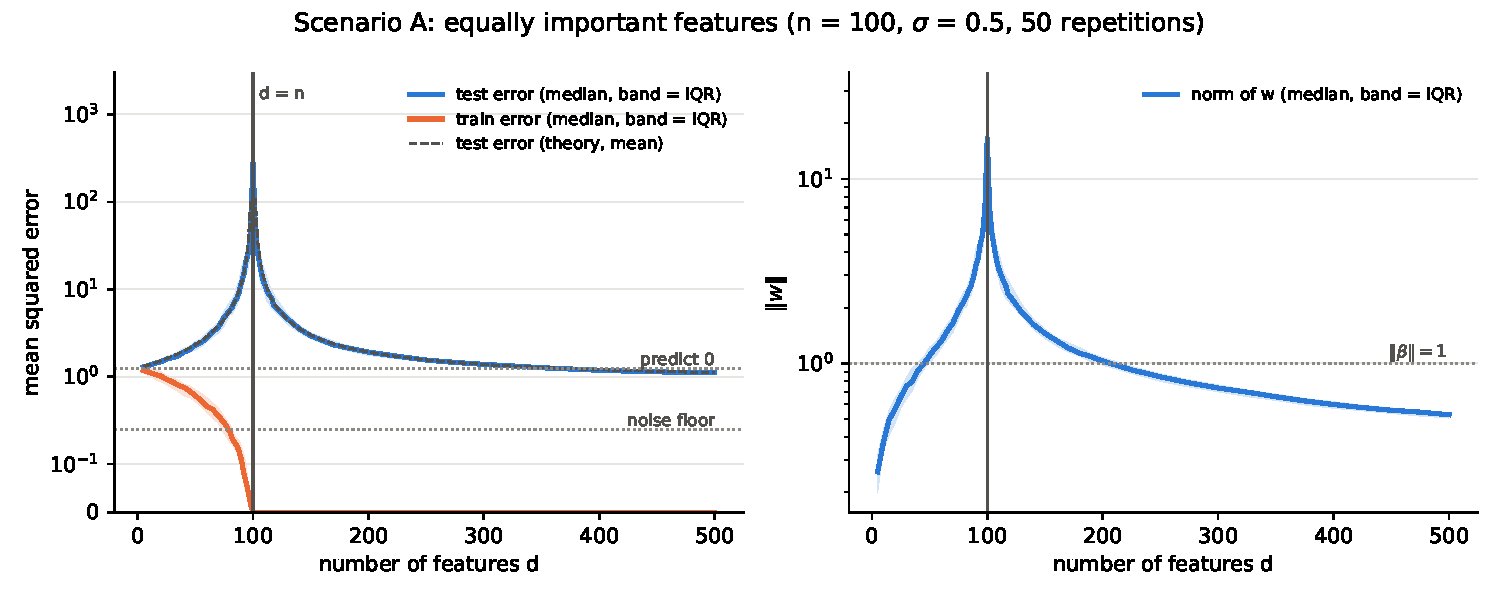
\includegraphics[width=0.68\linewidth]{synthetic_ls_A.pdf}\\[4pt]
  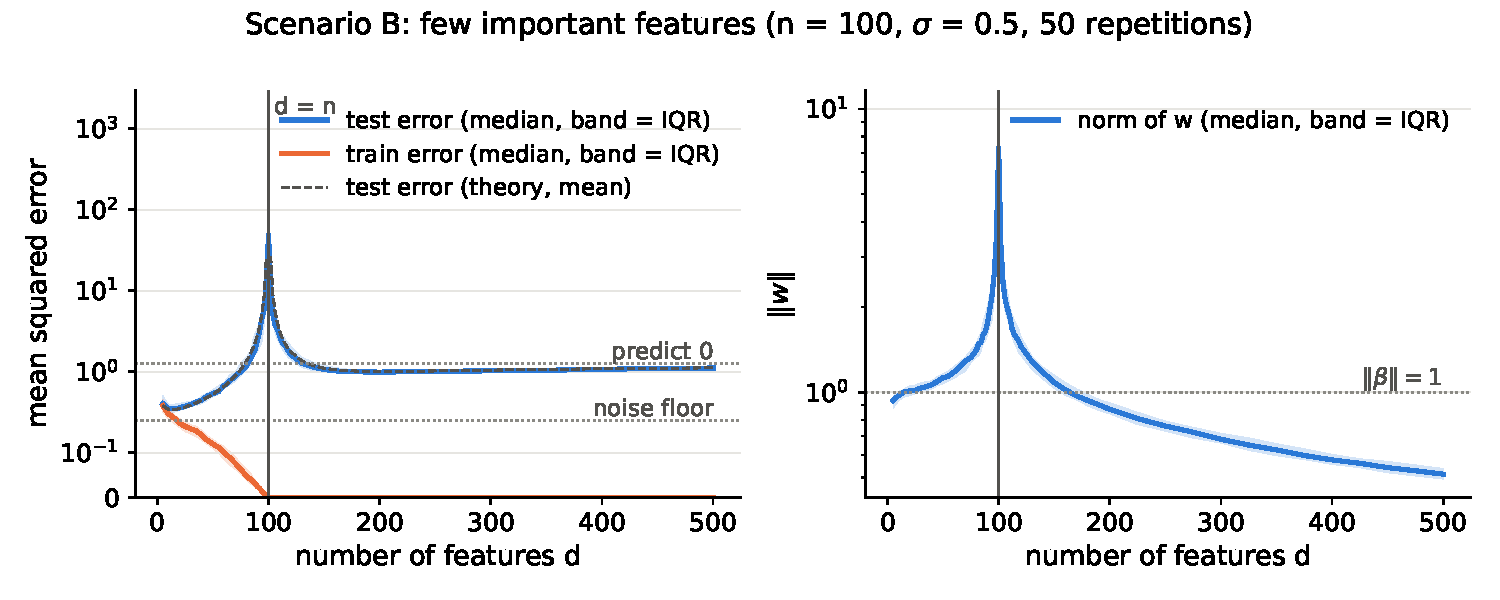
\includegraphics[width=0.68\linewidth]{synthetic_ls_B.pdf}
  \caption{Minimum-norm least squares on synthetic data (top: scenario A,
    bottom: scenario B). Left: median train and test error over 50
    repetitions, with interquartile band and the theoretical expected
    error (dashed). Right: norm of the estimated coefficients. The vertical
    line marks the interpolation threshold $d = n = 100$.}
  \label{fig:synthetic-ls}
\end{figure}

The theoretical curves of Equation~\eqref{eq:theory} follow the simulations
closely in both scenarios, which confirms the implementation. The two
scenarios differ in what happens away from the threshold. In
scenario A there is no classical U-shape: the test error grows from the
start, because each new feature adds very little signal and some variance.
After the threshold it keeps decreasing, and the best model is the largest
one, $d = 500$, with a median error of $1.10$. This is the main claim of
the paper: a model with five times more parameters than data points does
better than any model below the threshold. The gain, however, is small:
the trivial predictor that always outputs $0$ has error $1.25$. In
scenario B the U-shape appears: the error first goes down, reaching its
minimum of $0.35$ at $d = 15$, and then goes up. The second descent is
still there, but it never comes back below this minimum.

\subsection{Synthetic data: comparison with ridge}
Figure~\ref{fig:synthetic-ridge} compares least squares with ridge
regression. The larger $\lambda$, the lower the peak: in scenario A the
height of the peak (median test error) goes from $278$ with least squares to
$6.2$ with $\lambda = 1$, $2.4$ with $\lambda = 10$ and $1.3$ with
$\lambda = 100$. The norm of the coefficients, shown on the right, no longer
explodes. When $\lambda$ is chosen by cross-validation the peak disappears
completely and the test error stays almost flat as $d$ grows. In our
experiments, then, double descent is a property of the unregularized
estimator: with a well-chosen penalty there is no peak at all.

\begin{figure}[H]
  \centering
  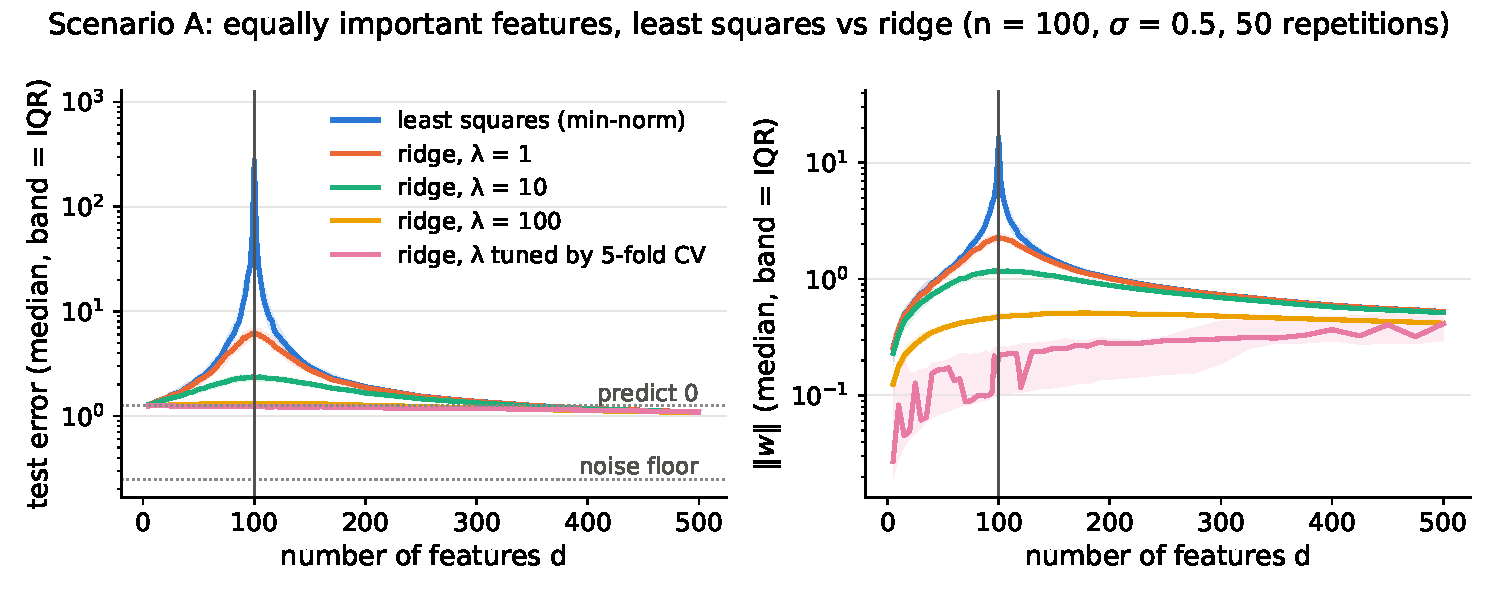
\includegraphics[width=0.68\linewidth]{synthetic_ridge_A.pdf}\\[4pt]
  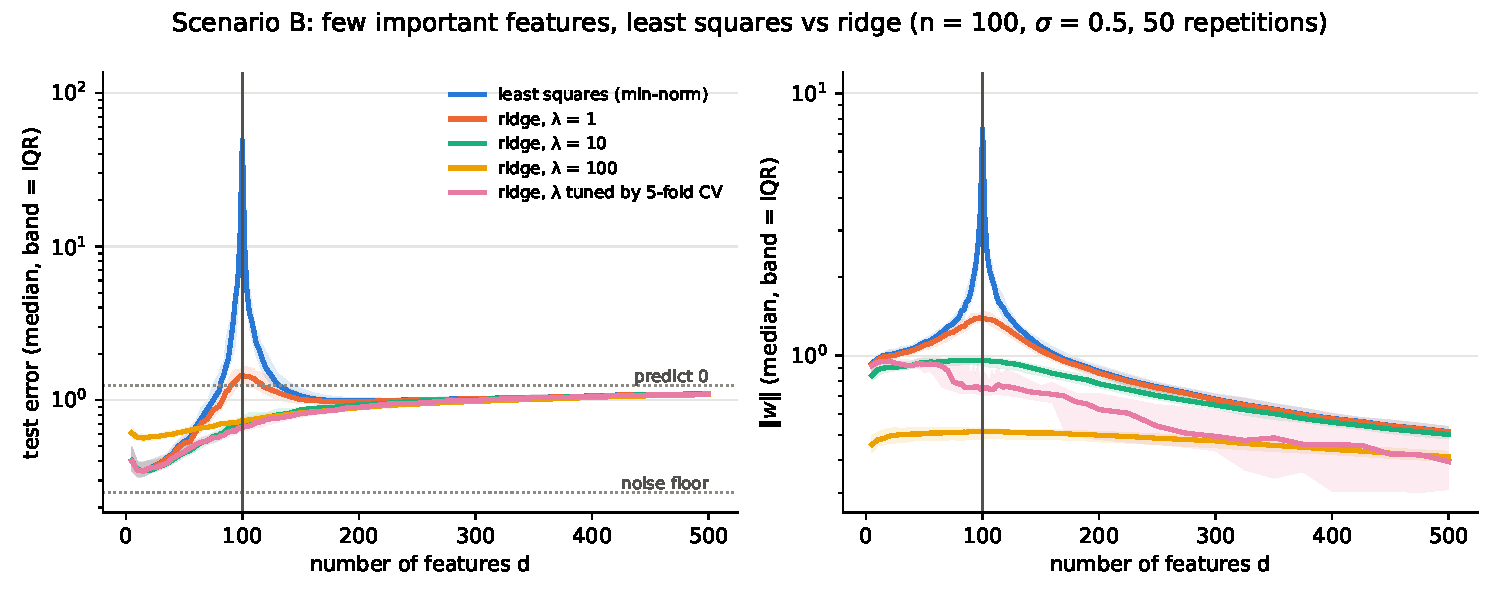
\includegraphics[width=0.68\linewidth]{synthetic_ridge_B.pdf}
  \caption{Least squares versus ridge regression on synthetic data (top:
    scenario A, bottom: scenario B). Left: median test error; right: norm
    of the coefficients. Ridge with $\lambda$ tuned by 5-fold
    cross-validation on the training set removes the peak.}
  \label{fig:synthetic-ridge}
\end{figure}

Far from the threshold all the methods give almost the same error (about
$1.1$ at $d = 500$ in scenario A): there the minimum-norm solution already
behaves like a regularized one. A penalty that is too strong also has a cost. In scenario B, where a few
features carry most of the signal, $\lambda = 100$ shrinks the important
coefficients as well, and the best error rises from $0.35$ to $0.57$. With
$\lambda$ chosen by cross-validation, instead, the best error is $0.34$,
the lowest of all. In scenario A the cross-validated model stays close to
the trivial predictor: with $100$
points and $500$ weak features there is little to learn, and
cross-validation detects it.

\subsection{Real data: California Housing}
On California Housing the picture is the same as on synthetic data
(Figure~\ref{fig:real-ls}). The training error reaches zero at $d = 100$,
the test error has a sharp peak at the same point, with a median of about
$4800$, and the norm of the coefficients peaks there too. After the
threshold the test error decreases again. Double descent therefore appears
on real data as well, with the threshold exactly at $d = n$.

\begin{figure}[H]
  \centering
  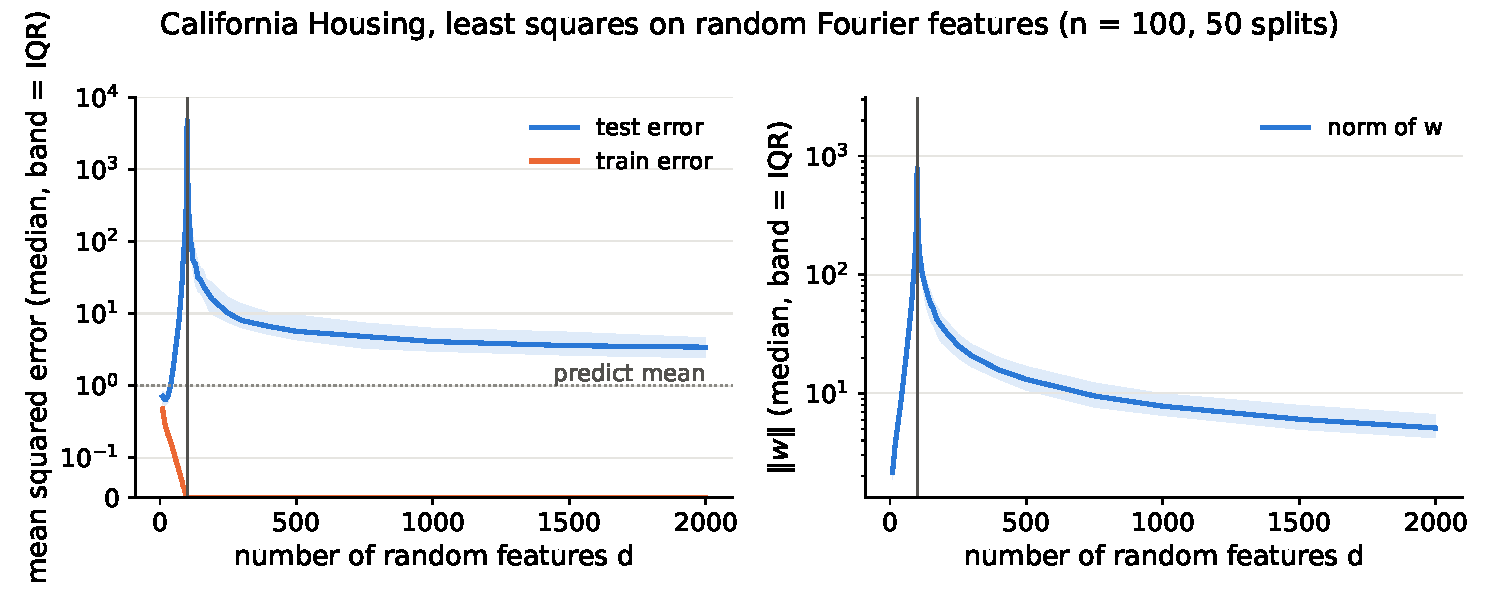
\includegraphics[width=0.8\linewidth]{real_ls.pdf}
  \caption{California Housing, minimum-norm least squares on random Fourier
    features (bandwidth from the median heuristic), 50 random train/test
    splits. Left: train and test error; right: norm of the coefficients.}
  \label{fig:real-ls}
\end{figure}

\begin{figure}[H]
  \centering
  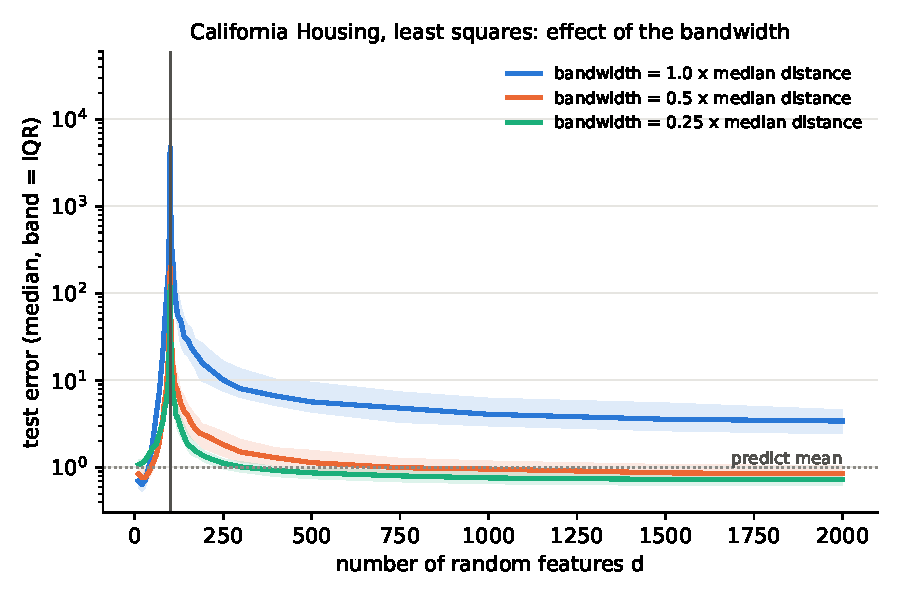
\includegraphics[width=0.5\linewidth]{real_bandwidth.pdf}
  \caption{California Housing, least squares with three bandwidths of the
    random features. Narrower features make the overparameterized regime
    competitive.}
  \label{fig:real-bandwidth}
\end{figure}

\begin{figure}[H]
  \centering
  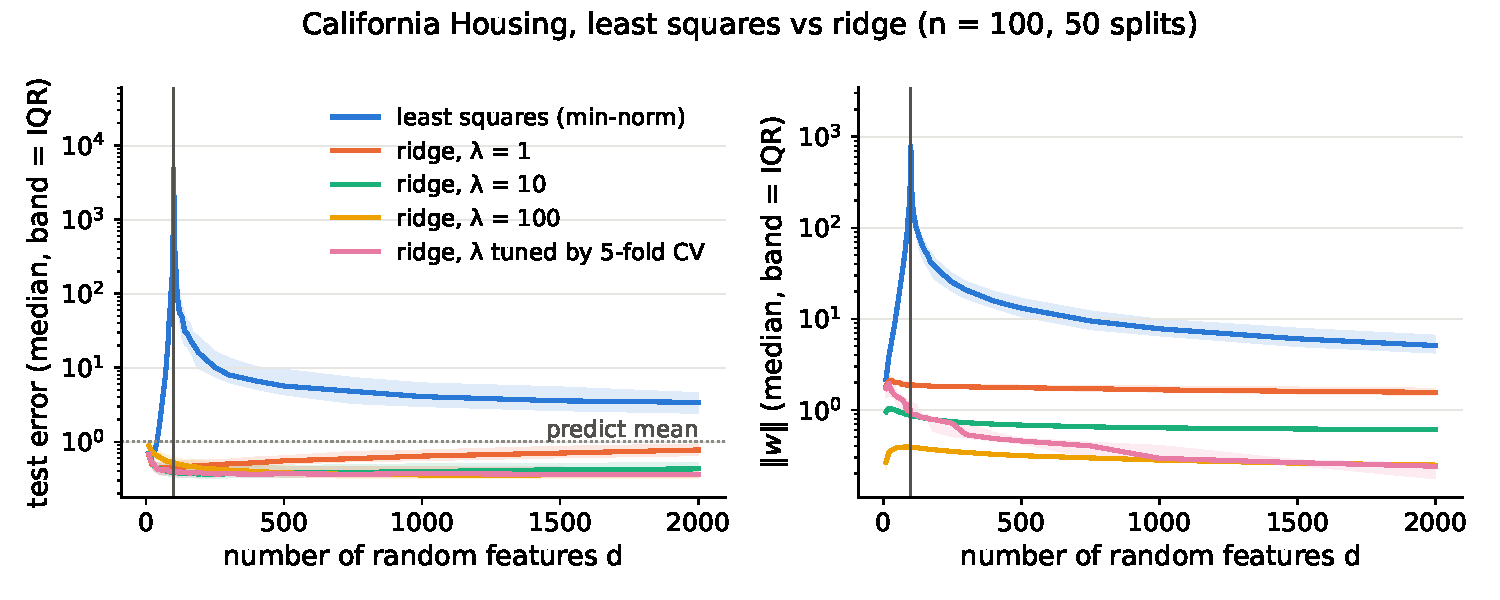
\includegraphics[width=0.8\linewidth]{real_ridge.pdf}
  \caption{California Housing, least squares versus ridge regression on the
    same random features.}
  \label{fig:real-ridge}
\end{figure}

With the bandwidth chosen by the median heuristic, however, the second
descent is not enough. The best model is a small one, $d = 20$, with a
median error of $0.63$, while at $d = 2000$ the error is still around $3$,
worse than predicting the mean. This is the same behaviour as scenario B.
Figure~\ref{fig:real-bandwidth} shows that the bandwidth changes this
conclusion. With narrower features ($h$ divided by $4$) the peak is much
lower and the error keeps decreasing up to $d = 2000$, where it reaches
$0.72$, below the trivial predictor and better than every model below the
threshold with the same bandwidth. Whether overparameterization pays off on
this dataset thus depends on how the features are built.

Ridge regression behaves as on synthetic data (Figure~\ref{fig:real-ridge}).
With $\lambda \ge 1$ the peak disappears, and with $\lambda$ chosen by
cross-validation the error keeps improving as features are added, down to
$0.36$ at $d = 1500$; ridge with $\lambda = 100$ does about as well
($0.357$ at $d = 1000$). The best results on this dataset are therefore
reached by strongly overparameterized models with the right amount of
regularization.

\subsection{Extension: gradient descent versus closed form}
Figure~\ref{fig:gd} compares gradient descent started at
$\mathbf{w} = \mathbf{0}$ with the closed-form solution. Away from the
threshold the two coincide: after $1000$ iterations the relative distance
between them is of order $10^{-15}$, both for $d < n$ and for $d > n$. So
for $d > n$ gradient descent finds exactly the minimum-norm interpolant,
even though nothing in the algorithm asks for it. This is the implicit
regularization of gradient descent: since every update is a combination of
the rows of $\mathbf{X}$, the iterates never leave the subspace that
contains the minimum-norm solution.

\begin{figure}[H]
  \centering
  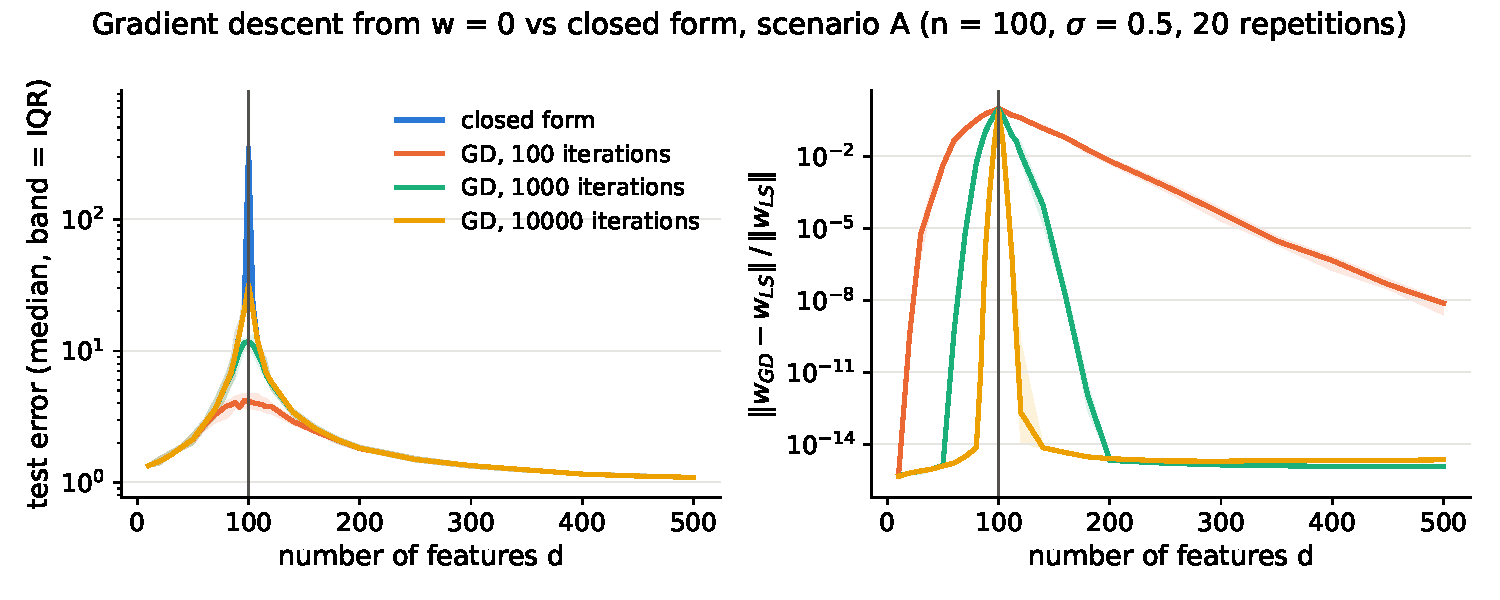
\includegraphics[width=0.8\linewidth]{synthetic_gd.pdf}
  \caption{Gradient descent started at $\mathbf{w} = \mathbf{0}$ versus the closed-form
    minimum-norm solution (scenario A, 20 repetitions). Left: median test
    error for three iteration budgets. Right: relative distance between the
    two solutions.}
  \label{fig:gd}
\end{figure}

Close to the threshold gradient descent does not converge in practice: at
$d = 100$ the relative distance is still $0.83$ after $10{,}000$
iterations. Convergence is slow there for the same reason the peak exists:
the smallest nonzero eigenvalue of $\mathbf{X}^\top \mathbf{X}$ is close to
zero, and along that direction each step moves very little. As a
consequence the peak of gradient descent is lower, and it grows with the
number of iterations: the median error at the threshold is about $4$ after
$100$ iterations, about $12$ after $1000$ and about $30$ after $10{,}000$,
against roughly $350$ for the closed form. Stopping early acts like ridge
regression: it prevents the coefficients from growing along the directions
where they would explode.

\subsection{Extension: effect of the label noise}
Figure~\ref{fig:noise} repeats the experiment on synthetic data with four
noise levels. More noise gives a higher peak in both scenarios: in
scenario B the median error at $d = n$ goes from $1.3$ without noise to
$15$, $49$ and $196$ for $\sigma = 0.25$, $0.5$ and $1$. Again, the
theoretical curves match the simulations.

\begin{figure}[H]
  \centering
  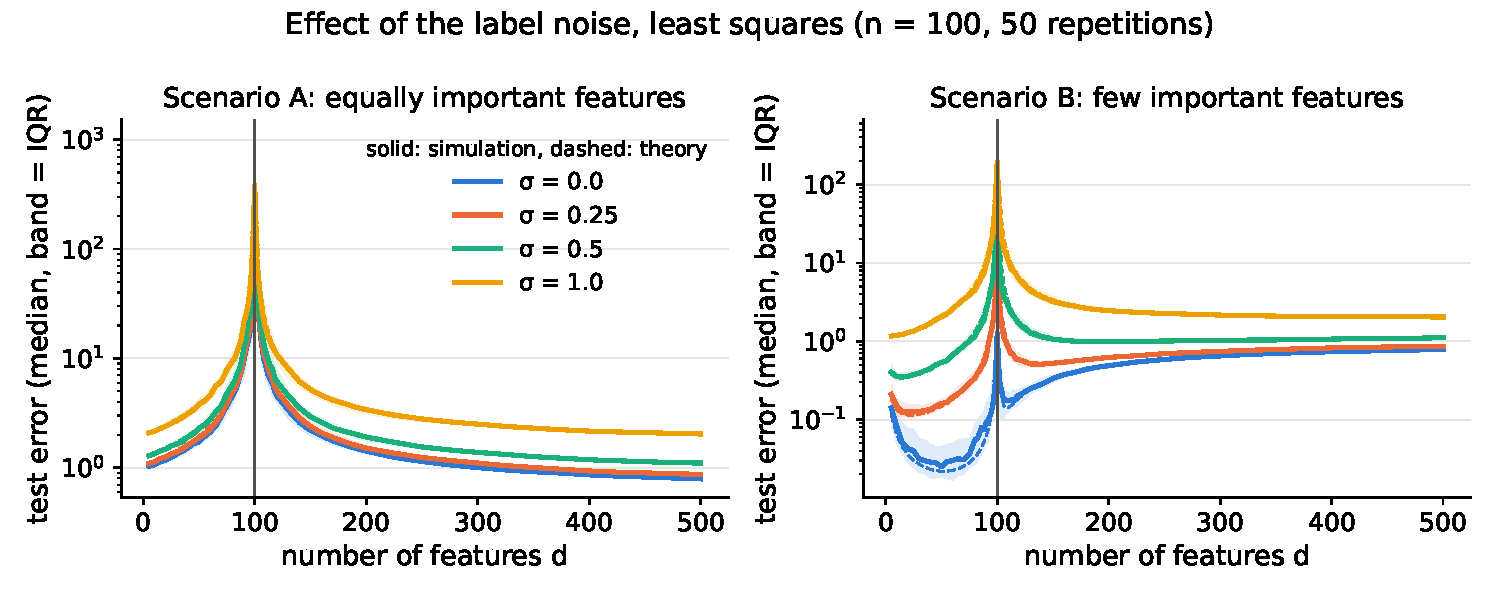
\includegraphics[width=0.8\linewidth]{synthetic_noise.pdf}
  \caption{Test error of minimum-norm least squares for four noise levels,
    simulation (solid) and theory (dashed).}
  \label{fig:noise}
\end{figure}

The two scenarios behave very differently when there is no noise. In
scenario B the peak almost disappears, because the first $100$ features
contain nearly all the signal and there is nothing left to fit by mistake.
In scenario A, instead, the peak is still large, about $179$, even with
$\sigma = 0$. The reason is that a model with $d = 100$ sees only a fifth
of the signal, and the rest acts as noise. Double descent therefore does
not require noise in the labels: it is enough that the model cannot
explain everything.

Noise also moves the best model. In scenario B the best $d$ goes from $50$
without noise to $15$ for $\sigma = 0.25$ and $\sigma = 0.5$, and to $5$
for $\sigma = 1$: the noisier the data, the smaller the model that works
best. Below the threshold the classical bias-variance trade-off still
holds.

% =================================================================== 6
\section{Discussion}

\paragraph{Where the classical picture fails.}
All our experiments show the same thing: beyond the interpolation threshold,
adding parameters does not make the model overfit more. The test error goes
down again, and in some settings (scenario A, California Housing with narrow
features) the best model of all has many more parameters than data points.
The classical view fails because it measures complexity by the number of
parameters. What actually drives the test error is the norm of the selected
solution: it peaks at $d = n$ exactly where the test error does, and it
decreases afterwards. The minimum-norm choice, whether made explicitly or
reached implicitly by gradient descent started at zero, acts as a
regularizer that the parameter count does not see.

\paragraph{Strengths.}
The threshold is always at $d = n$, on every dataset, noise level and
bandwidth, the simulations match the theory, and both extensions are
consistent with the main picture.

\paragraph{Limitations.}
The results also have clear limits. In scenario A the overparameterized
model wins, but only barely: its error is $1.10$, against $1.25$ for the
trivial predictor. In scenario B and on California Housing with the median
heuristic, the second descent never goes below the classical minimum, so
overparameterization is not always worth it. Moreover, ridge regression
with a cross-validated penalty removes the peak and is among the best
models in every setting: double descent is mostly a property of unregularized estimators,
and with a well-tuned regularizer the classical concern about the peak
disappears. Finally, our setting is narrow: a single training size
$n = 100$, Gaussian features in the synthetic experiments, a target that is
capped in California Housing, and on real data a dependence on the
bandwidth of the random features, which we fixed with a heuristic rather
than tuned.

\paragraph{Synthetic versus real data.}
The two datasets agree on the position of the peak, the behaviour of the
norm and the effect of ridge. They also agree on when overparameterization
helps: California Housing with the median heuristic behaves like
scenario B, and with narrower features like scenario A.


% =================================================================== 7
\section{Conclusion}

We reproduced the double descent curve for linear regression on synthetic
and real data, with the peak always at $d = n$. Overparameterized models can
beat the classical ones, but only when the signal is spread across many
features or the features are built appropriately, and a well-chosen ridge
penalty removes the peak. Double descent
does not overturn the bias--variance trade-off, but it shows that the
number of parameters is not the right measure of complexity: the norm of
the solution is.
% ================================================================= REFERENCES
\bibliographystyle{plain}
\bibliography{references}

% =============================================================== DECLARATION
\section*{Declaration}
I declare that this material, which I now submit for assessment, is entirely
my own work and has not been taken from the work of others, save and to the
extent that such work has been cited and acknowledged within the text of my
work. I understand that plagiarism, collusion, and copying are grave and
serious offences in the university and accept the penalties that would be
imposed should I engage in plagiarism, collusion or copying. This
assignment, or any part of it, has not been previously submitted by me or
any other person for assessment on this or any other course of study.


\end{document}